\documentclass{article}

\usepackage{../../header}

\geometry{
 a4paper,
 total={170mm,257mm},
 left=20mm,
 top=20mm,
 }

%%%%%%%%%%%%%%%%%%%%%%%%%%%%%%%%%%%%%%%%%%%%%%%%%%%%%%%%
%Preamble

\title{CAP Written Homework 10}
\author{Linden Disney-Hogg}
\date{April 2020}

%%%%%%%%%%%%%%%%%%%%%%%%%%%%%%%%%%%%%%%%%%%%%%%%%%%%%%%%
%%%%%%%%%%%%%%%%%%%%%%%%%%%%%%%%%%%%%%%%%%%%%%%%%%%%%%%%
\begin{document}
\maketitle

\section{Question 1}

In this question we are asked about the convergence of the series 
\eq{
\sum_{n=0}^\infty \frac{n^3 \cos(n\pi)}{n^4 + 3n^3+1}
}
A point I want to make is that issues of convergence of $\sum_n a_n$ only care about the long term behaviour of the sequence $a_n$. This is characterised precisely by the limit comparison theorem. For the sequence we are given, recognising that $cos(n\pi)=(-1)^n$, we get that the terms tend to $\frac{(-1)^n}{n}$. As such this entire question can be understood in terms of the properties of the alternating harmonic series. 

\section{Question 2}
We are then asked about the function given by 
\eq{
f(x) = \int_0^x \log(1+t^2) \, dt 
}

\subsection{Analytic solution}
The first thing to note about this function is that actually we can find a closed form expression for it (and congratulations to those of you who noticed this). This can be done by integration by parts 
\eq{
f(x) &= \int_0^x \log(1+t^2) \, dt \\
&= \psquare{t \log(1+t^2)}_0^x - \int_0^x t \cdot \frac{2t}{1+t^2} \, dt \\
&= x\log(1+x^2)-2 \int_0^x 1- \frac{1}{1+t^2} \, dt \\
&= x\log(1+x^2) - 2\int_0^x 1 -\frac{1}{1+t^2} \, dt \\
&= x\log(1+x^2) - 2\psquare{t-\arctan(t)}_0^x \\
&= x\log(1+x^2) + 2\psquare{\arctan(x)-x}
}
With this we could work out $f(1)$ exactly to be $\log(2)+\frac{\pi}{2}-2$.

\subsection{Bounding \secmath{f(1)}}
If we had not spotted the way to do the integral, we could try to come up with a sensible way to get some bounds on the value of $f(1)$. \\
First things first, we know $\forall t \in [0,1], \, \log(1+t^2) \geq 0$. As such we can immediately say $f(1) \geq 0$, giving a lower bound.\\
We can next calculate $\frac{d}{dt}\log(1+t^2) = \frac{2t}{1+t^2}$, which is again non-negative for $t \in [0,1]$. This gives us the very rough bound that 
\eq{
f(1) \leq \max_{t \in [0,1]} \log(1+t^2) = \log(2) = 0.69\dots
}
We can do even better than this bound. Note that $\frac{d^2}{dt^2} \log(1+t^2) = \frac{2(1-t^2)}{(1+t^2)^2}$, which is non-negative for $t\in(0,1)$. This means when we think about the graph of $\log(1+t^2)$, in the region $[0,1]$ is must lie below the straight line connecting $(0,0)$ and $(1,\log(2))$ as it is concave upwards. This immediately reduces our upper bound as we can bound $f(1)$ by the resulting area of the blue triangle in the figure. i.e. 
\eq{
f(1) \leq \frac{1}{2} \log(2) = 0.34\dots
} 
This concavity idea also lets me provide a sharper lower bound, by realising that the line tangent to $\log(1+t^2)$ at $t=1$ must lie below the curve in $[0,1]$. Hence we find a lower bound given by the green triangle in the figure. i.e. 
\eq{
f(1) \geq \frac{1}{2}\log(2)^2 = 0.24\dots
}
\begin{center}
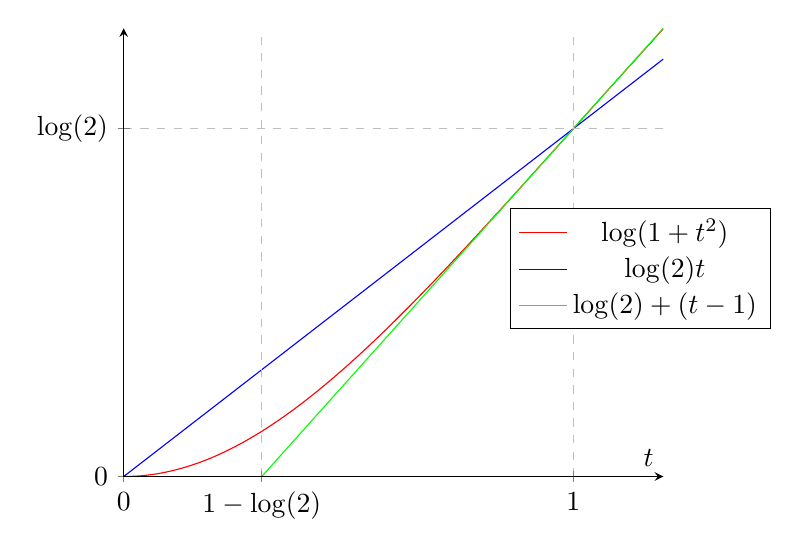
\begin{tikzpicture}
\begin{axis}[
axis lines = center,
xlabel = $t$,
legend style={at={(1.2,0.6)}},
xtick={0.307,1},
ytick={0.693},
xticklabels={$1-\log(2)$,$1$},
yticklabels={$\log(2)$},
ymajorgrids,
xmajorgrids,
grid style=dashed,
yticklabel pos=right,
extra x ticks={0},
extra y ticks = {0},
set layers,
axis on top,
]

\addplot [
domain=0:1.2, 
samples=100, 
color=red,
]
{ln(1+x^2)};
\addlegendentry{$\log(1+t^2)$}

\addplot [
domain=0:1.2, 
samples=100, 
color=blue,
]
{x*ln(2)};
\addlegendentry{$\log(2)t$}

\addplot [
domain=0.307:1.2,
samples=100,
color=green,
]
{ln(2)+x-1};
\addlegendentry{$\log(2)+(t-1)$}

\end{axis}
\end{tikzpicture}
\end{center}
This is already perhaps more work than is helpful, but if you are interested you can note that the choice of tangent line here was arbitary (I chose the tangent line to $t=1$ as it made the numbers easy), and any tangent line in the interval $[0,1]$ would have given a lower bound. Suppose we take the tangent at $t_0 \in [0,1]$. The tangent line here is given by 
\eq{
y = \log(1+t_0^2) + \frac{2t_0}{1+t_0^2}(t-t_0)
}
This line gives the lower bound 
\eq{
f(1) \geq \frac{1}{2} \psquare{\log(1+t_0^2) + \frac{2t_0(1-t_0)}{1+t_0^2}}\psquare{1-t_0 + \frac{(1+t_0^2)\log(1+t_0^2)}{2t_0}} = \frac{1+t_0^2}{4t_0}\psquare{\log(1+t_0^2) + \frac{2t_0(1-t_0)}{1+t_0^2}}^2
}
If you were interested you could find the maximum of this RHS bound on $[0,1]$, and it turns out it is $\approx 0.2473$, attained at $t_0 \approx 0.6297$, which is a slight improvement on taking $t_0=1$ ($\frac{1}{2}\log(2)^2 \approx 0.2402$).

\subsection{Validity of power series}
The question asks you to find the power series for $f(x)$. There are two ways to do this 
\begin{enumerate}
	\item Plug in the power series for $x\log(1+x^2) + 2\psquare{\arctan(x)-x}$ after having solved the integral exactly.
	\item Integrate term by term the power series the power series 
	\eq{
\log(1+t^2) = \sum_{n=1}^\infty (-1)^{n-1} \frac{t^{2n}}{n}	
}
\end{enumerate}
The written solutions expect you to do the second method, so it is worth thinking about the subtleties involved in this method. \\
Using what we know about the convergence of series, we can see that this power series converges iff $\abs{t}\leq 1$. This means that if we used the second method to find the power series for $f(x)$ when $\abs{x}>1$, it would have to fail. Fortunately when we are asked to work out $f(1)$, the integral only covers a region where the power series is valid, so we can carry on. \\
Now at some point in the calculation we have to make the equality 
\eq{
\int_0^1 \sum_{n=1}^\infty (-1)^n \frac{t^{2n}}{n} \, dt = \sum_{n=1}^\infty \int_0^1  (-1)^n \frac{t^{2n}}{n} \, dt 
}
This would be fine if the sum was finite, but knowing now that we have to be careful with limits, we can ask whether this interchange of sum and integral is always valid? The answer is no, and we can choose a simple counter example. Let $a_0(t)=1$ on $[0,1]$, and 
\eq{
a_n(t) = \left\lbrace \begin{array}{cc}
	-n & \frac{1}{n+1} < t \leq \frac{1}{n} \\
	1 & \text{otherwise}
\end{array} \right.
}
for $n \geq 1$ Then 
\eq{
\sum_{n=0}^{N-1} a_n(t) = \left\lbrace \begin{array}{cc}
	N & 0 \leq t \leq \frac{1}{N} \\
	0 & \text{otherwise}
\end{array} \right.
}
For any $t$ this series converges with
\eq{
\sum_{n \geq 0} a_n(t) = 0
}
(just choose $N>t$) and so 
\eq{
\int_0^1 \sum_{n \geq 0} a_n(t) \, dt = 0
}
Now 
\eq{
\int_0^1 a_0(t) \, dt &= 1 \\
\text{for }n \geq 1, \, \int_0^1 a_n(t) \, dt &=\frac{1}{n+1} -n\pround{\frac{1}{n} - \frac{1}{n+1}}  = 0
}
so 
\eq{
\sum_{n \geq 0} \int_0^1 a_n(t) \, dt = 1
}
It turns out we can rectify this problem if the series is absolutely convergent and we are integrating over a finite region, as in the case of question 2. I will not prove this, but if you are interested you should look into measure theory. 
\begin{comment}
\subsection{Swapping sums and integrals - an example}
Let me define a function $a$ by 
\eq{
a(t) = \left\lbrace \begin{array}{cc}
\sin(\pi t) & 0 \leq t \leq 1 \\
0 & \text{otherwise}
\end{array} \right.
}
$a(t)$ looks like half a single period of a sin function in the interval $[0,1]$. Now let me define $a_n(t)$ by 
\eq{
a_n(t) = b_n a(t-n) - b_{n+1} a(t-n-1)
}
where $b_n$ is some other real sequence. The $a_n$ for $b_n = \frac{1}{n}$ are displayed below. 

\begin{center}
	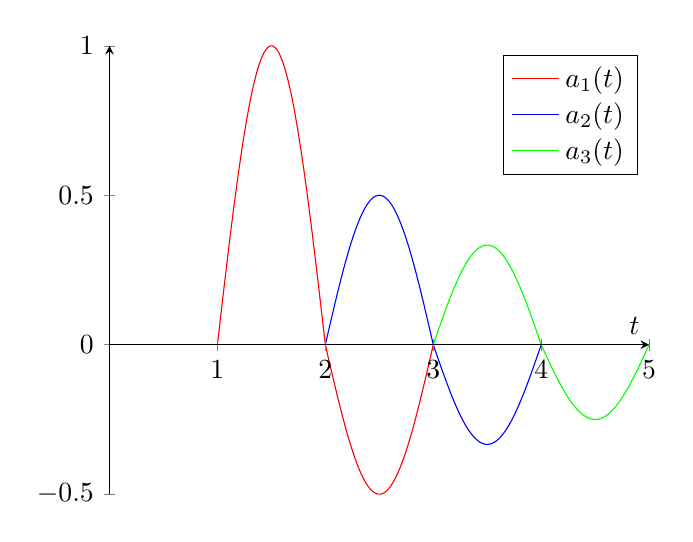
\begin{tikzpicture}
	\begin{axis}[
	axis lines = center,
	xlabel = $t$,
	xmin = 0,
	%legend style={at={(1.2,0.6)}},
	%xtick={1},
	%ytick={0.693},
	%yticklabels={$\log(2)$},
	%ymajorgrids,
	%xmajorgrids,
	%grid style=dashed,
	%yticklabel pos=right,
	%extra x ticks={0},
	extra y ticks = {0},
	set layers,
	axis on top,
	]
	
	
	\addplot [
	domain=1:2, 
	samples=100, 
	color=red,
	]
	{sin(deg(pi*(x-1)))};
	\addlegendentry{$a_1(t)$}
	
		\addplot [
	domain=2:3, 
	samples=100, 
	color=red,
	forget plot,
	]
	{-sin(deg(pi*(x-2)))/2};
	
		
	\addplot [
	domain=2:3, 
	samples=100, 
	color=blue,
	]
	{sin(deg(pi*(x-2)))/2};
	\addlegendentry{$a_2(t)$}
	
	\addplot [
	domain=3:4, 
	samples=100, 
	color=blue,
	forget plot,
	]
	{-sin(deg(pi*(x-3)))/3};
	
		\addplot [
	domain=3:4, 
	samples=100, 
	color=green,
	]
	{sin(deg(pi*(x-3)))/3};
	\addlegendentry{$a_3(t)$}
	
	\addplot [
	domain=4:5, 
	samples=100, 
	color=green,
	forget plot,
	]
	{-sin(deg(pi*(x-4)))/4};
	
	\end{axis}
	\end{tikzpicture}
\end{center}

We can now define functions $g_N$ by 
\eq{
g_N(t) = \sum_{n=1}^{N-1} a_n(t) = b_1 a(t-1) -b_N a(t-N)
}
\end{comment}

\end{document}
